\documentclass[11pt,a4paper]{article}

\usepackage[T1]{fontenc}
\usepackage[utf8]{inputenc}
\usepackage{lmodern}
\usepackage{mathptmx}
\usepackage[Symbol]{upgreek}
\usepackage[margin=2.3cm]{geometry}
\usepackage{microtype}
\usepackage{amsmath,amssymb,amsthm}
\usepackage{graphicx}
\usepackage{booktabs}
\usepackage{tabularx}
\usepackage{enumitem}
\usepackage{float}
\usepackage[font=small,labelfont=bf]{caption}
\usepackage[hidelinks]{hyperref}

\setlength{\parindent}{0pt}
\setlength{\parskip}{6pt}
\linespread{1.08}
\setlist{itemsep=2pt,topsep=3pt}

% Auto-generated by make_paper_assets.py -- do not edit by hand.
\newcommand{\bestLeakDeadPct}{96}
\newcommand{\bestLeakLambda}{10}
\newcommand{\bestLeakMode}{mean}
\newcommand{\bestLeakRouting}{0.0003}
\newcommand{\bestLeakValue}{0.0020}
\newcommand{\bestRoutAlivePct}{83}
\newcommand{\bestRoutLeak}{0.296}
\newcommand{\bestRoutValue}{0.40}
\newcommand{\blockOffPositive}{4}
\newcommand{\blockPositive}{19}
\newcommand{\blockRuns}{5}
\newcommand{\blockSig}{10}
\newcommand{\blockSigHolm}{1}
\newcommand{\blockSigTauFifty}{1}
\newcommand{\blockSigTauFive}{3}
\newcommand{\blockSigTauTen}{4}
\newcommand{\blockSigTauTwenty}{2}
\newcommand{\blockSignP}{2.0\times10^{-5}}
\newcommand{\blockTotal}{20}
\newcommand{\budget}{10}
\newcommand{\cgGptSent}{+0.109}
\newcommand{\cgGptTox}{+0.133}
\newcommand{\cgPGptSent}{$<$0.001}
\newcommand{\cgPGptTox}{0.879}
\newcommand{\cgPQwenSent}{0.004}
\newcommand{\cgPQwenTox}{0.007}
\newcommand{\cgQwenSent}{+0.277}
\newcommand{\cgQwenTox}{+0.127}
\newcommand{\contrastFVUlamOne}{0.250}
\newcommand{\contrastFVUlamTen}{1.03}
\newcommand{\contrastRoutLamOne}{0.36}
\newcommand{\degenCorrMax}{-0.28}
\newcommand{\dimGptSent}{+0.404}
\newcommand{\dimGptTox}{+0.130}
\newcommand{\dimQwenSent}{+0.413}
\newcommand{\dimQwenTox}{+0.044}
\newcommand{\dimSentSAEbetter}{0}
\newcommand{\dimSentSAEworse}{12}
\newcommand{\dimSentTotal}{12}
\newcommand{\dimToxSAEbetter}{3}
\newcommand{\dimToxSAEworse}{0}
\newcommand{\dimToxTotal}{8}
\newcommand{\dissBUnw}{-0.447}
\newcommand{\dissBWan}{+0.184}
\newcommand{\dissGUnw}{+0.183}
\newcommand{\dissGWan}{-0.411}
\newcommand{\dissRUnw}{-0.039}
\newcommand{\dissRWan}{+0.001}
\newcommand{\evVanGPT}{80}
\newcommand{\evVanQwen}{96}
\newcommand{\fvuCGGPT}{0.277}
\newcommand{\fvuCGQwen}{0.066}
\newcommand{\fvuVanGPT}{0.203}
\newcommand{\fvuVanQwen}{0.045}
\newcommand{\layerDisagree}{4}
\newcommand{\layerFracMax}{85}
\newcommand{\layerFracMin}{27}
\newcommand{\layerGptAUC}{0.816}
\newcommand{\layerGptLoss}{45}
\newcommand{\layerGptProbe}{11}
\newcommand{\layerGptSteer}{7}
\newcommand{\layerScans}{4}
\newcommand{\leakRatioBestVsRout}{146}
\newcommand{\leakRoutingCorr}{+0.03}
\newcommand{\nPrimaryRuns}{5}
\newcommand{\nRuns}{6}
\newcommand{\nSynthSeeds}{20}
\newcommand{\penformConfigs}{12}
\newcommand{\penformSeeds}{2}
\newcommand{\qtoxLfifteenEff}{+0.062}
\newcommand{\qtoxLfifteenPPL}{37.6}
\newcommand{\qtoxLtenEff}{+0.056}
\newcommand{\qtoxLtenPPL}{6.5}
\newcommand{\scarGptSent}{+0.118}
\newcommand{\scarGptTox}{+0.194}
\newcommand{\scarPGptSent}{$<$0.001}
\newcommand{\scarPGptTox}{0.022}
\newcommand{\scarPQwenSent}{$<$0.001}
\newcommand{\scarPQwenTox}{0.075}
\newcommand{\scarQwenSent}{+0.147}
\newcommand{\scarQwenTox}{+0.075}
\newcommand{\specMax}{16.6}
\newcommand{\specMaxBuf}{4.33}
\newcommand{\specMaxLamFive}{14.0}
\newcommand{\specNoBufLamFive}{0.91}
\newcommand{\specNoBufLamOne}{1.5}
\newcommand{\specOffMax}{1.65}
\newcommand{\specOffMin}{0.99}
\newcommand{\sqFVUspread}{1.2\times10^{-4}}
\newcommand{\sqLeakLamThirty}{0.435}
\newcommand{\sqLeakLamZero}{0.495}
\newcommand{\sqPenShare}{0.5}
\newcommand{\sqPenTermThirty}{8.7\times10^{-4}}
\newcommand{\sqRoutMax}{0.012}
\newcommand{\synthBAliveMin}{100}
\newcommand{\synthRouting}{0.35}
\newcommand{\synthRoutingOff}{0.010}
\newcommand{\vanFVUpenform}{0.173}
\newcommand{\vsSSVgptPmax}{0.40}
\newcommand{\vsSSVgptPmin}{0.24}
\newcommand{\vsSSVgptPositive}{3}
\newcommand{\vsSSVgptSig}{0}
\newcommand{\vsSSVgptTotal}{4}
\newcommand{\vsSSVqwenPositive}{8}
\newcommand{\vsSSVqwenPrimSig}{4}
\newcommand{\vsSSVqwenPrimTotal}{6}
\newcommand{\vsSSVqwenSig}{6}
\newcommand{\vsSSVqwenSigHolm}{3}
\newcommand{\vsSSVqwenTotal}{8}
\newcommand{\vsScarQwenSig}{1}
\newcommand{\vsScarSig}{1}
\newcommand{\vsScarTotal}{12}

% Auto-generated by make_ea_assets.py -- do not edit by hand.
\newcommand{\ghBadGen}{+0.111}
\newcommand{\ghBadNeg}{+30.1}
\newcommand{\ghBadNegHi}{+31.7}
\newcommand{\ghBadNegLo}{+28.4}
\newcommand{\ghBadPos}{+9.1}
\newcommand{\ghGoodGen}{+0.092}
\newcommand{\ghGoodNeg}{+6.7}
\newcommand{\ghGoodNegHi}{+7.2}
\newcommand{\ghGoodNegLo}{+6.5}
\newcommand{\ghGoodPos}{+26.6}
\newcommand{\ghRandGen}{+0.078}
\newcommand{\ghRandNeg}{+9.7}
\newcommand{\ghRandNegHi}{+14.6}
\newcommand{\ghRandNegLo}{+6.6}
\newcommand{\ghRandPos}{+11.1}
\newcommand{\ghRelearnBad}{0.54}
\newcommand{\ghRelearnRand}{0.52}
\newcommand{\ghRouting}{0.37}
\newcommand{\ghSeeds}{3}
\newcommand{\ghWikiBucket}{120}
\newcommand{\ghWikiCostPct}{105}
\newcommand{\ghWikiPlain}{59}
\newcommand{\glBadGen}{-0.028}
\newcommand{\glBadNeg}{+9.0}
\newcommand{\glBadNegHi}{+9.0}
\newcommand{\glBadNegLo}{+9.0}
\newcommand{\glBadPos}{+8.6}
\newcommand{\glGoodGen}{-0.055}
\newcommand{\glGoodNeg}{+8.3}
\newcommand{\glGoodNegHi}{+8.3}
\newcommand{\glGoodNegLo}{+8.2}
\newcommand{\glGoodPos}{+8.1}
\newcommand{\glRandGen}{+0.022}
\newcommand{\glRandNeg}{+9.3}
\newcommand{\glRandNegHi}{+10.6}
\newcommand{\glRandNegLo}{+8.0}
\newcommand{\glRandPos}{+9.1}
\newcommand{\glRelearnBad}{0.67}
\newcommand{\glRelearnRand}{0.68}
\newcommand{\glRouting}{0.00}
\newcommand{\glSeeds}{3}
\newcommand{\glWikiBucket}{59}
\newcommand{\glWikiPlain}{59}
\newcommand{\gtBadGen}{+0.048}
\newcommand{\gtBadNeg}{+26.5}
\newcommand{\gtBadNegHi}{+29.2}
\newcommand{\gtBadNegLo}{+24.8}
\newcommand{\gtBadPos}{+9.6}
\newcommand{\gtGoodGen}{+0.080}
\newcommand{\gtGoodNeg}{+7.7}
\newcommand{\gtGoodNegHi}{+7.9}
\newcommand{\gtGoodNegLo}{+7.6}
\newcommand{\gtGoodPos}{+21.6}
\newcommand{\gtRandGen}{+0.085}
\newcommand{\gtRandNeg}{+10.5}
\newcommand{\gtRandNegHi}{+13.0}
\newcommand{\gtRandNegLo}{+7.5}
\newcommand{\gtRandPos}{+12.2}
\newcommand{\gtRelearnBad}{0.63}
\newcommand{\gtRelearnRand}{0.63}
\newcommand{\gtRouting}{0.29}
\newcommand{\gtSeeds}{3}
\newcommand{\gtWikiBucket}{69}
\newcommand{\gtWikiCostPct}{19}
\newcommand{\gtWikiPlain}{58}
\newcommand{\slBadGen}{-0.011}
\newcommand{\slBadNeg}{+19.7}
\newcommand{\slBadNegHi}{+21.2}
\newcommand{\slBadNegLo}{+18.3}
\newcommand{\slBadPos}{+7.3}
\newcommand{\slGoodGen}{-0.040}
\newcommand{\slGoodNeg}{+6.9}
\newcommand{\slGoodNegHi}{+9.2}
\newcommand{\slGoodNegLo}{+4.5}
\newcommand{\slGoodPos}{+26.3}
\newcommand{\slRandGen}{+0.001}
\newcommand{\slRandNeg}{+0.2}
\newcommand{\slRandNegHi}{+0.3}
\newcommand{\slRandNegLo}{+0.1}
\newcommand{\slRandPos}{+0.1}
\newcommand{\slRelearnBad}{0.74}
\newcommand{\slRelearnRand}{0.74}
\newcommand{\slRouting}{0.87}
\newcommand{\slSeeds}{2}
\newcommand{\slWikiBucket}{1932}
\newcommand{\slWikiPlain}{1957}
\newcommand{\ssBadGen}{-0.116}
\newcommand{\ssBadNeg}{+3.9}
\newcommand{\ssBadNegHi}{+4.6}
\newcommand{\ssBadNegLo}{+3.2}
\newcommand{\ssBadPos}{-0.4}
\newcommand{\ssGoodGen}{+0.064}
\newcommand{\ssGoodNeg}{-0.3}
\newcommand{\ssGoodNegHi}{+0.1}
\newcommand{\ssGoodNegLo}{-0.8}
\newcommand{\ssGoodPos}{+3.4}
\newcommand{\ssRandGen}{-0.020}
\newcommand{\ssRandNeg}{+0.5}
\newcommand{\ssRandNegHi}{+0.5}
\newcommand{\ssRandNegLo}{+0.4}
\newcommand{\ssRandPos}{+0.4}
\newcommand{\ssRelearnBad}{0.67}
\newcommand{\ssRelearnRand}{0.62}
\newcommand{\ssRouting}{0.92}
\newcommand{\ssSeeds}{2}
\newcommand{\ssWikiBucket}{7208}
\newcommand{\ssWikiPlain}{12579}


% IEEEtran.bst control entry under the article class
\makeatletter
\def\bstctlcite{\@ifnextchar[{\@bstctlcite}{\@bstctlcite[@auxout]}}
\def\@bstctlcite[#1]#2{\@bsphack
  \@for\@citeb:=#2\do{%
    \edef\@citeb{\expandafter\@firstofone\@citeb}%
    \if@filesw\immediate\write\csname #1\endcsname{\string\citation{\@citeb}}\fi}%
  \@esphack}
\makeatother

\newtheorem{proposition}{Proposition}
\theoremstyle{definition}
\newtheorem{definition}{Definition}

\newcommand{\Wb}{\mathrm{W}}
\newcommand{\Nb}{\mathrm{N}}
\newcommand{\Ub}{\mathrm{U}}
\newcommand{\avg}{\operatorname{mean}}
\newcommand{\why}[1]{\par\smallskip\noindent\textbf{Rationale.}\enspace #1\par}

\begin{document}
\bstctlcite{IEEEexample:BSTcontrol}

\begin{center}
{\LARGE\bfseries Technical Notes}\\[6pt]
{\large Localising Unwanted Knowledge in Language Models\\ with Reserved Buckets and a Neutral Buffer}\\[10pt]
Varanasi Sathveek, Vanamala Aravind, Pula Naga Manikanta, K.\ Hima Bindu\\
{\small Department of Computer Science \& Engineering, NIT Andhra Pradesh}\\[4pt]
{\small Companion to the CARE 2026 extended abstract}\\[2pt]
{\small Code and results: \url{https://github.com/VSathveek/Research_On_Mechanistic_Interpretability/tree/main/cgsae}}
\end{center}

\bigskip
\noindent\textbf{Main results at a glance.}
\begin{center}
\small
\begin{tabularx}{\linewidth}{>{\raggedright\arraybackslash}p{4.2cm}>{\raggedright\arraybackslash}X}
\toprule
Claim & Evidence\\
\midrule
The buffer is what makes deletion targeted & Toy model: specificity \specMax$\times$ with a wide
buffer, \specNoBufLamFive{} (chance) without it; \nSynthSeeds{} seeds.\\
Unwanted knowledge can be placed and removed inside a pretrained LM & GPT-2, $\uplambda=3$: deleting
$\Ub$ raises perplexity on negative reviews by \gtBadNeg\% vs \gtBadPos\% on positive, in
\gtSeeds{}/\gtSeeds{} seeds; random deletion is symmetric.\\
Same pattern when training from scratch & Larger scratch model: \slBadNeg\% vs \slBadPos\%;
random deletion \slRandNeg\%.\\
Reserved SAE bucket beats a random block & \blockPositive{} of \blockTotal{} settings, sign test
$p=\blockSignP$.\\
Competitive with SOTA steering on toxicity & Qwen2.5-1.5B: \cgQwenTox{} vs \dimQwenTox{} for
difference-in-means (CAA-style), $p=\cgPQwenTox$ (about $2.9\times$).\\
Common metric is misleading & Leakage vs routing: $r=\leakRoutingCorr$; best-leakage bucket is
\bestLeakDeadPct\% dead.\\
\bottomrule
\end{tabularx}
\end{center}

\tableofcontents
\newpage

%=====================================================================
\section{Problem statement}
\label{sec:problem}

A language model sometimes produces things we do not want, for example toxic language. We would
like to remove that behaviour while leaving everything else the model knows untouched.

This is hard because of \emph{superposition}~\cite{elhage2022toy}. A model has to represent far more
concepts than it has neurons. It solves this by letting each neuron take part in many concepts,
and each concept spread over many neurons. So there is usually no single place to cut.
If we switch off neurons involved in toxicity, we also damage other things those neurons help with.


Existing approaches deal with this \emph{after} the model is trained:
\begin{itemize}
  \item \textbf{Activation steering} finds a direction in the model's hidden space linked to a
  behaviour and adds or removes it at run time~\cite{turner2023actadd,rimsky2024caa,li2023iti,zou2023repe}.
  \item \textbf{Sparse autoencoders (SAEs)} split the hidden state into many simpler features,
  and people then search for the features linked to a behaviour~\cite{bricken2023monosemanticity,cunningham2024sparse,gao2024scaling}.
  Supervised versions tie a behaviour to one chosen feature (SCAR~\cite{harle2024scar}) or
  select features with labels (SAE-SSV~\cite{he2025saessv}).
  \item \textbf{Gradient routing}~\cite{cloud2024gradient} goes furthest: it masks gradients during
  training so that a capability is learned in a chosen part of the network.
\end{itemize}

\textbf{Our question.} Can we decide \emph{before training} where an unwanted behaviour will live,
so that it can later be removed by simply deleting that location? And what should happen to the
features that both the wanted and the unwanted behaviour need (for example, general grammar or
words like ``movie'' that appear in both positive and negative reviews)?

\textbf{Our answer, in one sentence.} Reserve one bucket of units for the unwanted behaviour, one
for the wanted behaviour, and leave a \emph{neutral buffer} between them for shared features;
train with a penalty that rewards each bucket for carrying its own behaviour; then delete the
unwanted bucket.

%=====================================================================
\section{Background}
\label{sec:background}

\subsection{Hidden units, layers and the MLP}
A transformer language model such as GPT-2~\cite{radford2019gpt2} processes text token by token.
At each layer every token has a hidden vector $\mathbf h\in\mathbb R^{d}$ (for GPT-2 small,
$d=768$). Each layer contains an MLP (a small two-layer neural network):
\begin{equation}
  \mathrm{MLP}(\mathbf h)=W_{\mathrm{out}}\,\upphi\!\big(W_{\mathrm{in}}\mathbf h+\mathbf b_{\mathrm{in}}\big)+\mathbf b_{\mathrm{out}},
\end{equation}
where $W_{\mathrm{in}}\in\mathbb R^{m\times d}$, $W_{\mathrm{out}}\in\mathbb R^{d\times m}$ and
$\upphi$ is the GELU activation. The $m$ entries of $\upphi(\cdot)$ are the \emph{MLP neurons}. In GPT-2,
$m=4d=3072$. In the GPT-2 code these weights are called \texttt{c\_fc} and \texttt{c\_proj}.

\subsection{Superposition}
If a layer has $m$ neurons but must represent $F\gg m$ concepts, the concepts cannot each have
their own neuron. Elhage et al.~\cite{elhage2022toy} showed that networks then store concepts as
nearly-orthogonal directions that overlap. Neuron $j$ ends up responding to several unrelated
concepts (it is \emph{polysemantic}). This is the reason that deleting neurons is usually not
targeted.

\subsection{Sparse autoencoders (SAEs)}
An SAE is a second network trained to rewrite a hidden vector $\mathbf x\in\mathbb R^{d}$ as a
sparse combination of many more features ($m>d$). We use the TopK SAE of Gao et
al.~\cite{gao2024scaling,makhzani2013ksparse}:
\begin{align}
  \mathbf z&=\mathrm{TopK}_k\!\Big(\mathrm{ReLU}\big(W_{\mathrm{enc}}(\mathbf x-\mathbf b_{\mathrm{pre}})+\mathbf b_{\mathrm{enc}}\big)\Big),\\
  \hat{\mathbf x}&=W_{\mathrm{dec}}\mathbf z+\mathbf b_{\mathrm{pre}}.
\end{align}
$\mathrm{TopK}_k$ keeps the $k$ largest entries and sets the rest to zero, so exactly $k$ features
are active per token ($L_0=k$). Each column $\mathbf w_j$ of $W_{\mathrm{dec}}$ is the direction
of feature $j$. The SAE is trained to make $\hat{\mathbf x}$ close to $\mathbf x$, measured by the
\emph{fraction of variance unexplained}:
\begin{equation}
  \mathrm{FVU}=\frac{\sum_t\|\mathbf x_t-\hat{\mathbf x}_t\|^2}{\sum_t\|\mathbf x_t-\bar{\mathbf x}\|^2}.
\end{equation}
FVU $=0$ is perfect; FVU $=1$ is no better than predicting the average.

Our settings: $k=32$; width $m=8d$ (6144 features for GPT-2, 12288 for Qwen2.5-1.5B~\cite{qwen2024qwen25}).

\why{TopK fixes the number of active features, so every SAE we compare has exactly the same
sparsity. With an $L_1$ penalty instead, sparsity would differ between runs and comparisons would
be unfair. Width $8d$ is a standard choice that fits our compute budget.}

\subsection{Activation steering and difference-in-means}
The simplest steering method takes the mean hidden vector on unwanted texts minus the mean on
wanted texts,
\begin{equation}
  \mathbf v=\avg_{y=0}\mathbf h-\avg_{y=1}\mathbf h,
\end{equation}
and subtracts a multiple of it at run time: $\mathbf h'=\mathbf h-\upbeta\,\hat{\mathbf v}$. This is
the idea behind ActAdd~\cite{turner2023actadd} and contrastive activation addition
(CAA)~\cite{rimsky2024caa}; a single such direction even controls refusal in chat
models~\cite{arditi2024refusal}. It is a strong and cheap baseline, so we always compare against it.

\subsection{Perplexity}
Perplexity measures how surprised a model is by a text:
\begin{equation}
  \mathrm{PPL}=\exp\!\Big(-\frac1T\sum_{t=1}^{T}\log p(x_t\mid x_{<t})\Big).
\end{equation}
Lower is better. If deleting a bucket makes perplexity on negative reviews rise a lot, but on
positive reviews only a little, then the deleted bucket held knowledge that was specific to
negative text. This is how we measure \emph{knowledge removal}. We report the rise in percent:
$100\,(\mathrm{PPL}_{\text{after}}/\mathrm{PPL}_{\text{before}}-1)$.

\subsection{AUC}
The area under the ROC curve (AUC) is the probability that a randomly chosen positive example is
scored higher than a randomly chosen negative one. $0.5$ is chance; $1$ is perfect. We use it in
the toy experiment because, unlike accuracy, it does not depend on a decision threshold.

%=====================================================================
\section{Our method: buckets and a neutral buffer}
\label{sec:method}

\subsection{The partition}
Take a layer with $m$ hidden units (MLP neurons inside a language model, or features inside an
SAE). Choose a fraction $\uptau$ with $0<\uptau\le\frac12$ and let $n=\lfloor\uptau m\rfloor$.
Before training we fix three index sets:
\begin{equation}
  \Wb=\{0,\dots,n-1\},\qquad
  \Nb=\{n,\dots,m-n-1\},\qquad
  \Ub=\{m-n,\dots,m-1\}.
\end{equation}
$\Wb$ is the \emph{wanted bucket}, $\Ub$ the \emph{unwanted bucket}, and $\Nb$ the
\emph{neutral buffer}. The buffer has $m-2n$ units, and we call
\begin{equation}
  \uprho=\frac{m-2n}{2n}
\end{equation}
the buffer ratio. At $\uptau=\frac12$ we get $\uprho=0$: no buffer. At $\uptau=0.1$ we get
$\uprho=4$: the buffer is four times as big as both buckets together.

\why{The floor $\lfloor\cdot\rfloor$ is there only because the number of units must be a whole
number. $\uptau$ cannot exceed $\frac12$ because two buckets of size $\uptau m$ must fit inside $m$
units. Choosing contiguous index ranges is just a convention; any fixed choice works because the
units start out symmetric.}

\subsection{Labels}
Each training text has a label $y$: $y=0$ for unwanted (for example a negative review or a toxic
comment), $y=1$ for wanted. Every token inherits the label of its text, as in
SCAR~\cite{harle2024scar}. Labels are used \emph{only} inside the training penalty; the model never
sees them as input.

\subsection{The share of activity in a bucket}
For a token with unit activations $a_1,\dots,a_m\ge0$ (for MLP neurons we clamp negatives to zero),
the share of activity in a set $S$ is
\begin{equation}
  s_S=\frac{\sum_{j\in S}a_j}{\sum_{j=1}^{m}a_j+\upepsilon},
\end{equation}
with a tiny $\upepsilon$ to avoid division by zero. Shares lie between $0$ and $1$.

\subsection{The contrastive penalty}
We train with $L=L_{\text{task}}+\uplambda P$, where $L_{\text{task}}$ is the usual loss (next-token
loss for a language model, FVU for an SAE, cross-entropy for the toy classifier) and
\begin{equation}
  \boxed{\;P=-\tfrac12\Big[\big(\avg_{y=0}s_{\Ub}-\avg_{y=1}s_{\Ub}\big)+\big(\avg_{y=1}s_{\Wb}-\avg_{y=0}s_{\Wb}\big)\Big].\;}
  \label{eq:P}
\end{equation}
The averages are over tokens of each class in the mini-batch.


\textbf{Range of $P$.} Each share is in $[0,1]$, so each bracket is in $[-1,1]$ and
$P\in[-1,1]$. Two cases matter:
\begin{itemize}
  \item If both buckets are \emph{silent} (shares always $0$), then $P=0$.
  \item If routing is \emph{perfect} ($\Ub$ takes all activity on unwanted text and none on wanted
  text, and the reverse for $\Wb$), then $P=-1$.
\end{itemize}
So silence is \emph{not} a good solution: it scores $0$, while real routing scores close to $-1$.
This is the key difference from the penalty we started with (Section~\ref{sec:penform}).

\subsection{Why the neutral buffer is needed}
Many features are useful for both classes: grammar, punctuation, the word ``film'', and so on.
Without a buffer, every unit belongs to $\Wb$ or $\Ub$, so a shared feature must sit in one of the
buckets. If it sits in $\Ub$, deleting $\Ub$ damages wanted text too; if it sits in $\Wb$, the
penalty pushes against it. With a buffer, shared features have a third place to go that is never
penalised and never deleted. Experiment~1 tests this directly.

\why{This is the central idea of the project. Superposition means shared features are unavoidable;
the buffer gives them a home so that the buckets can be clean.}

\subsection{Deleting the unwanted bucket}
\textbf{Inside a model.} For each bucketed layer we zero the weights that feed into and out of
every neuron $j\in\Ub$:
\begin{equation}
  W_{\mathrm{in}}[j,:]=0,\qquad b_{\mathrm{in}}[j]=0,\qquad W_{\mathrm{out}}[:,j]=0 .
\end{equation}
(In the GPT-2 code, which stores these as \texttt{Conv1D}, this is \texttt{c\_fc.weight[:,U]},
\texttt{c\_fc.bias[U]} and \texttt{c\_proj.weight[U,:]}.) The neurons are then gone: they can no
longer affect the output.

\textbf{Inside an SAE.} The language model itself is frozen; the SAE only reads its hidden vector
$\mathbf h$. We scale the $\Ub$ features by $(1-\upalpha)$ with $\upalpha\in[0,1]$, and add only the
\emph{change} this makes:
\begin{equation}
  \mathbf z'_{\Ub}=(1-\upalpha)\,\mathbf z_{\Ub},\qquad
  \mathbf h'=\mathbf h+\upsigma\big(\hat{\mathbf x}(\mathbf z')-\hat{\mathbf x}(\mathbf z)\big)
  =\mathbf h-\upalpha\,\upsigma\sum_{j\in\Ub}z_j\,\mathbf w_j ,
  \label{eq:delta}
\end{equation}
where $\upsigma$ undoes the scaling we applied to activations before training the SAE.

\why{If we replaced $\mathbf h$ by the SAE's reconstruction $\hat{\mathbf x}$, every edit would
also pay the SAE's reconstruction error, even at $\upalpha=0$. With the difference form,
$\upalpha=0$ changes nothing at all, so the cost we measure is the cost of the edit alone.}

%=====================================================================
\section{How we measure success}
\label{sec:metrics}

\begin{definition}[Specificity, toy experiment]
Let $\Delta\mathrm{AUC}_{\Ub}$ be the drop in the classifier's AUC for recognising the unwanted
class when $\Ub$ is deleted, and $\Delta\mathrm{AUC}_{\mathrm{rand}}$ the drop when a random set of
the same size is deleted. Then
\begin{equation}
  S=\frac{\Delta\mathrm{AUC}_{\Ub}}{\Delta\mathrm{AUC}_{\mathrm{rand}}} .
\end{equation}
$S=1$ means $\Ub$ is no more targeted than any random set of units. $S=10$ means deleting $\Ub$
hurts the unwanted class ten times more than deleting a random set of the same size.
\end{definition}

\why{Deleting units always hurts something. Without the random-set control, ``deleting $\Ub$ hurts
the unwanted class'' could just mean ``deleting any 12 units hurts''. The ratio removes that
confusion. Our preliminary (minor-project) version lacked this control; adding it was the first fix.}

\begin{definition}[Selective knowledge loss, in-model]
After deleting a bucket we measure the perplexity rise on held-out \emph{negative} reviews and on
held-out \emph{positive} reviews. Deleting $\Ub$ should raise the first much more than the second;
deleting $\Wb$ should do the reverse; deleting a random bucket should raise both about equally.
\end{definition}

\begin{definition}[Routing]
$R=\avg_{y=0}s_{\Ub}-\avg_{y=1}s_{\Ub}$ on held-out text: how much more of the activity $\Ub$
carries on unwanted text than on wanted text. $R\approx0$ means no bucket has formed.
\end{definition}

\begin{definition}[Behaviour]
We generate continuations of review openings with greedy decoding and score them with a sentiment
classifier (DistilBERT fine-tuned on SST-2~\cite{sanh2019distilbert,socher2013sst}). For toxicity
we use a RoBERTa toxicity classifier~\cite{logacheva2022paradetox}. The behaviour score is the
fraction of continuations judged negative (or toxic).
\end{definition}

\begin{definition}[Relearning]
After deletion we fine-tune for 100 steps on negative reviews and measure the negative-generation
rate again. If it returns to the same level as after deleting a random bucket, the knowledge was
removed but can be relearned.
\end{definition}

\begin{definition}[Effect at a matched fluency budget, SAE experiments]
For each method we try several strengths. For each strength $i$ we record the effect $e_i$ (how
much the unwanted score falls) and the fluency cost
$q_i=100(\mathrm{PPL}_i/\mathrm{PPL}_0-1)$ on WikiText-103~\cite{merity2017wikitext}. We sort by
cost, take the best effect reached so far at each cost (the upper envelope
$\tilde e_i=\max_{j\le i}e_j$), and read off the effect at cost $b=\budget\%$:
$E_{\budget}=\mathrm{interp}(\budget;\{q_i\},\{\tilde e_i\})$.
\end{definition}

\why{Any method can reduce toxicity by breaking the model; a broken model says nothing toxic. So
we compare all methods at the \emph{same} damage to fluency. This is fairer than comparing at the
same strength, because a strength of 1 means different things for different methods.}

\textbf{Statistics.} Comparisons over seeds use paired $t$-tests. Where many tests are run together,
we correct with Holm--Bonferroni~\cite{holm1979}. For ``does $\Ub$ beat a random bucket across
all 20 settings'' we use a \emph{sign test}: if there were no real effect, each setting would be a
coin flip, so getting $\blockPositive$ wins out of $\blockTotal$ has probability $p=\blockSignP$.

\subsection{Why we stopped trusting ``leakage''}
\label{sec:leakage}
The usual measure for this kind of method is \emph{leakage}: how much $\Ub$ fires on wanted text and
$\Wb$ fires on unwanted text. Low leakage looks good. But a bucket that never fires at all has zero
leakage. We checked this across \penformConfigs{} configurations: leakage and routing had
correlation $r=\leakRoutingCorr$, i.e.\ none. The configuration with the best leakage had
\bestLeakDeadPct\% of its unwanted bucket dead (never firing) and routing
$R=\bestLeakRouting$. This is why we report routing and occupancy instead
(Figure~\ref{fig:penform}).

%=====================================================================
\section{From the first penalty to the contrastive penalty}
\label{sec:penform}

The minor-project version used a \emph{squared-mean} penalty. Writing $\bar a_S$ for the mean
activation over units in $S$:
\begin{equation}
  P_{\mathrm{sq}}=\big(\avg_{y=0}\bar a_{\Wb}\big)^2+\big(\avg_{y=1}\bar a_{\Ub}\big)^2 .
\end{equation}
It punishes each bucket for firing on the \emph{wrong} class. Two problems appeared.

\textbf{Problem 1: it barely works when activity is sparse.} In a TopK SAE only $k=32$ of the $m$
units are active per token. With $n=1228$ units in a bucket, the bucket mean is of order $10^{-2}$,
its square of order $10^{-4}$, and the gradient reaching any one unit is divided again by $n$. In
our calibration, raising $\uplambda$ from $0$ to $30$ moved normalised leakage only from
\sqLeakLamZero{} to \sqLeakLamThirty{} (random is $0.5$). The minor project did not see this
because its autoencoder was dense (about 394 of 768 units active).

\textbf{Problem 2: it can be satisfied by doing nothing.}

\begin{proposition}[Silent buckets are a perfect score for suppression penalties]
Suppose a penalty only punishes $\Wb$ firing on unwanted text and $\Ub$ firing on wanted text, is
never negative, and is zero when both are silent. If the buffer has at least $k$ units, then a
model that uses only the buffer and leaves both buckets silent has penalty $0$, the minimum, for
any $\uplambda$.
\end{proposition}
\begin{proof}[Reason]
If neither bucket ever fires, the punished quantities are zero, so the penalty is zero. The
remaining loss is that of an ordinary SAE built from the buffer units, which is possible because
the buffer has at least $k$ units.
\end{proof}


The contrastive penalty~\eqref{eq:P} fixes both problems. It uses \emph{shares}, which do not
shrink with sparsity, and it \emph{rewards} a bucket for carrying its own class, so silence
($P=0$) is worse than routing ($P\to-1$).

\begin{figure}[H]
  \centering
  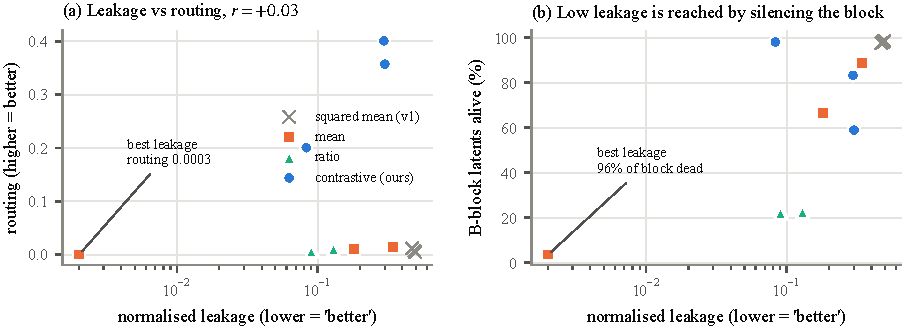
\includegraphics[width=0.95\linewidth]{figures/fig_penform.pdf}
  \caption{Penalty forms on GPT-2 SAEs (\penformConfigs{} configurations, $\uptau=0.20$,
  \penformSeeds{} seeds each). (a) Leakage does not track routing. (b) The lowest-leakage
  configurations reach it by silencing the unwanted bucket.}
  \label{fig:penform}
\end{figure}

%=====================================================================
\section{Experiment 1: the toy model}
\label{sec:exp1}

\textbf{Setup.} Two classes of 64-dimensional points drawn from overlapping Gaussians (500
training and 1000 test points). A two-layer network with 32 hidden units classifies them, with the
hidden units split into $\Wb$, $\Nb$ and $\Ub$. Training: Adam, learning rate $0.01$, 200 epochs.
We vary $\uptau\in\{0.1,\dots,0.5\}$ and $\uplambda\in\{0,1,5\}$, with \nSynthSeeds{} seeds each.

\why{A toy model lets us change one thing at a time (buffer size, penalty strength) and run many
seeds cheaply on a CPU. It is where the idea can be checked cleanly before spending GPU time.}

\textbf{Results} (Table~\ref{tab:spec}, Figure~\ref{fig:toy}).
\begin{itemize}
  \item Without the penalty ($\uplambda=0$), $S$ stays between \specOffMin{} and \specOffMax{}:
  just reserving indices does nothing.
  \item With the penalty and a wide buffer ($\uptau=0.1$, buffer ratio $4.33$), $S$ reaches
  \specMax{} at $\uplambda=1$ and \specMaxLamFive{} at $\uplambda=5$.
  \item As the buffer shrinks, $S$ falls. With no buffer ($\uptau=\frac12$), $S$ is
  \specNoBufLamOne{} at $\uplambda=1$ and \specNoBufLamFive{} at $\uplambda=5$, i.e.\ chance.
  \item Deleting $\Ub$ destroys the unwanted class and deleting $\Wb$ the wanted class; a random
  set does neither (Figure~\ref{fig:toy}b).
\end{itemize}

\begin{table}[H]
\centering
\caption{Specificity $S$ in the toy model (mean over \nSynthSeeds{} seeds).}
\label{tab:spec}
\begin{tabular}{ccccc}
\toprule
$\uptau$ & buffer ratio $\uprho$ & $S$ at $\uplambda=0$ & $S$ at $\uplambda=1$ & $S$ at $\uplambda=5$\\
\midrule
0.1 & 4.33 & 1.65 & 16.6 & 14.0\\
0.2 & 1.67 & 1.26 & 3.96 & 4.76\\
0.3 & 0.78 & 1.11 & 1.61 & 2.52\\
0.4 & 0.33 & 0.99 & 1.63 & 1.67\\
0.5 & 0    & 1.07 & 1.47 & 0.91\\
\bottomrule
\end{tabular}
\end{table}

\begin{figure}[H]
  \centering
  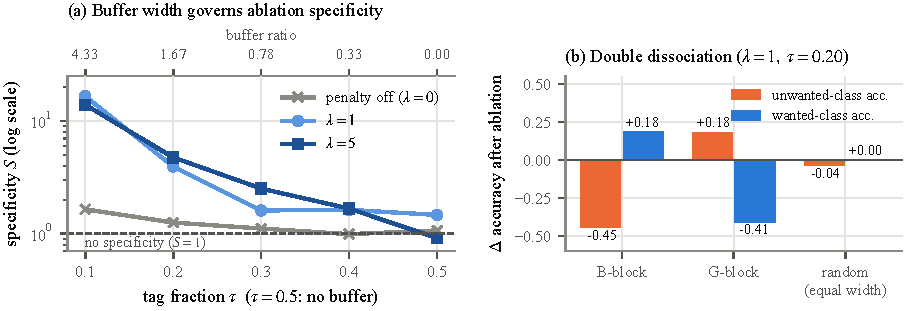
\includegraphics[width=0.95\linewidth]{figures/fig_synthetic.pdf}
  \caption{Toy model. (a) Specificity against tag fraction. With the penalty off, $S\approx1$
  everywhere; with it on, $S$ is largest with a wide buffer and returns to chance without one.
  (b) At $\uplambda=1,\uptau=0.2$ each bucket selectively destroys its own class; a random set does
  neither.}
  \label{fig:toy}
\end{figure}

\textbf{What we learn.} The penalty is needed (no penalty, no effect) and the buffer is needed (no
buffer, no effect). This is the cleanest evidence for the central idea.

%=====================================================================
\section{Experiment 2: buckets inside a real language model}
\label{sec:exp2}

\textbf{Setup.}
\begin{itemize}
  \item \textbf{Data:} IMDB movie reviews~\cite{maas2011imdb}. Negative sentiment is the unwanted
  behaviour ($y=0$), positive is wanted ($y=1$).
  \item \textbf{Fine-tuning:} GPT-2 small, buckets on the MLP neurons of layers 5--9 ($m=3072$
  per layer, $\uptau=0.1$, so 307 neurons per bucket per layer). 600 steps, batch 16, AdamW,
  learning rate $5\times10^{-5}$, $\uplambda\in\{1,3,10\}$, 3 seeds.
  \item \textbf{From scratch:} a small GPT-style model (6 layers, width 256) and a larger one,
  buckets on layers 1--4, 4000 steps, batch 32, learning rate $6\times10^{-4}$, 2 seeds.
  \item \textbf{Measured:} perplexity on held-out negative and positive reviews; WikiText-103
  perplexity for general fluency; behaviour (negative-generation rate); relearning.
  \item \textbf{Controls:} delete $\Wb$; delete a random set of the same size; a plain model trained
  without buckets.
\end{itemize}

\why{The SAE version (Experiment 3) only edits a frozen model from outside. The original idea was
to place the buckets \emph{inside} the model and delete real weights. Fine-tuning GPT-2 tests this
on a real pretrained model; training from scratch tests whether buckets form more easily when the
model learns everything with the penalty from the start. Layers 5--9 are the middle five of GPT-2's
twelve layers, away from the input embedding and the output; layers 1--4 cover most of the small
model.}

\textbf{Results} (Table~\ref{tab:inmodel}, Figure~\ref{fig:inmodel}).

\begin{table}[H]
\centering
\caption{Perplexity rise (\%) on held-out negative / positive reviews after deleting each bucket.
Mean over seeds.}
\label{tab:inmodel}
\small
\begin{tabular}{lcccccc}
\toprule
Setting & seeds & routing $R$ & delete $\Ub$ & delete $\Wb$ & delete random & fluency (Wiki PPL)\\
\midrule
GPT-2, $\uplambda=1$  & \glSeeds & \glRouting & \glBadNeg{} / \glBadPos & \glGoodNeg{} / \glGoodPos & \glRandNeg{} / \glRandPos & \glWikiBucket{} vs \glWikiPlain\\
GPT-2, $\uplambda=3$  & \gtSeeds & \gtRouting & \gtBadNeg{} / \gtBadPos & \gtGoodNeg{} / \gtGoodPos & \gtRandNeg{} / \gtRandPos & \gtWikiBucket{} vs \gtWikiPlain\\
GPT-2, $\uplambda=10$ & \ghSeeds & \ghRouting & \ghBadNeg{} / \ghBadPos & \ghGoodNeg{} / \ghGoodPos & \ghRandNeg{} / \ghRandPos & \ghWikiBucket{} vs \ghWikiPlain\\
Scratch, small & \ssSeeds & \ssRouting & \ssBadNeg{} / \ssBadPos & \ssGoodNeg{} / \ssGoodPos & \ssRandNeg{} / \ssRandPos & --\\
Scratch, large & \slSeeds & \slRouting & \slBadNeg{} / \slBadPos & \slGoodNeg{} / \slGoodPos & \slRandNeg{} / \slRandPos & --\\
\bottomrule
\end{tabular}
\end{table}

How to read the table:
\begin{itemize}
  \item At $\uplambda=1$ no bucket forms ($R=\glRouting$), and all three deletions do the same thing.
  \item At $\uplambda=3$ the pattern appears in all \gtSeeds{} seeds: deleting $\Ub$ raises perplexity
  on negative reviews by \gtBadNeg\% (range \gtBadNegLo{} to \gtBadNegHi) but on positive reviews by
  only \gtBadPos\%. Deleting $\Wb$ does the reverse. A random set hurts both about equally. The
  price is general fluency: WikiText perplexity is \gtWikiBucket{} instead of \gtWikiPlain{}
  (\gtWikiCostPct\% worse).
  \item At $\uplambda=10$ the pattern is stronger (\ghBadNeg\% vs \ghBadPos\%) but fluency costs
  \ghWikiCostPct\%. So $\uplambda=3$ is the best trade-off we found.
  \item The larger from-scratch model shows the same pattern (\slBadNeg\% vs \slBadPos\%), with
  random deletion almost harmless. (Perplexities of the from-scratch models are high because they
  are tiny and briefly trained; only the comparison between deletions matters.)
\end{itemize}

\begin{figure}[H]
  \centering
  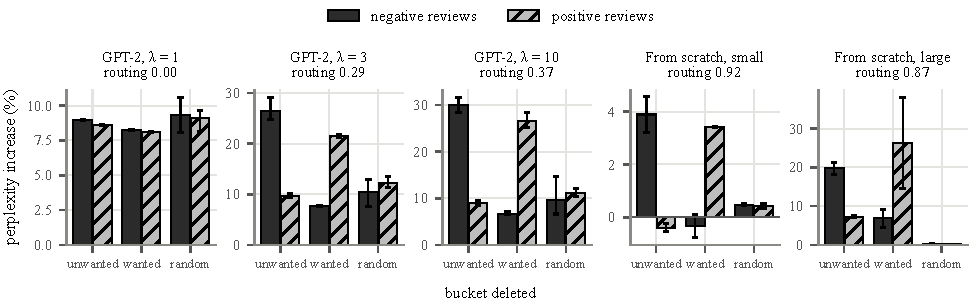
\includegraphics[width=0.98\linewidth]{figures/fig_inmodel.pdf}
  \caption{Perplexity rise on held-out reviews after deleting a bucket, for each setting.}
  \label{fig:inmodel}
\end{figure}

\textbf{Behaviour and relearning.} Removing knowledge did not reliably change what the model
\emph{writes}. The change in negative-generation rate after deleting $\Ub$ was \gtBadGen{} for GPT-2
($\uplambda=3$) and \slBadGen{} for the large scratch model; only the small scratch model showed a
clear drop (\ssBadGen, 2 seeds). After 100 steps of retraining, the negative-generation rate was
\gtRelearnBad{} after deleting $\Ub$ and \gtRelearnRand{} after deleting a random set: the
knowledge comes back as easily.

\textbf{What we learn.} The knowledge of an unwanted behaviour can be placed in a chosen location and
removed selectively, as measured by perplexity. Changing behaviour is harder; that is our next step.

%=====================================================================
\section{Experiment 3: buckets inside sparse autoencoders}
\label{sec:exp3}

\textbf{Setup.}
\begin{itemize}
  \item \textbf{Models:} GPT-2 small and Qwen2.5-1.5B-Instruct, both frozen.
  \item \textbf{Concepts:} sentiment (IMDB~\cite{maas2011imdb}) and toxicity
  (RealToxicityPrompts~\cite{gehman2020rtp}).
  \item \textbf{SAEs:} TopK, $k=32$, width $8d$, trained on 300{,}000 tokens from 6000 documents for
  30 epochs; $\uptau\in\{0.05,0.1,0.2,0.5\}$; 3 seeds.
  \item \textbf{Layers:} chosen by scanning every layer (Section~\ref{sec:layers}): GPT-2 layer 7
  (sentiment) and 8 (toxicity); Qwen layers 15 and 18 (sentiment), 10 and 15 (toxicity).
  \item \textbf{Compared methods, all at a \budget\% fluency budget:} our bucketed SAE (CG-SAE)
  deleting $\Ub$; the same SAE deleting a random block; a normal SAE with features chosen afterwards
  using labels (in the style of SAE-SSV~\cite{he2025saessv}); one conditioned feature
  (SCAR~\cite{harle2024scar}); difference-in-means steering and a linear-probe direction.
\end{itemize}

\why{The SAE version lets us work with a pretrained model that we cannot retrain, including a
1.5B-parameter model that would not fit in our GPU budget for fine-tuning. Two models and two
concepts test whether the result generalises. Comparing at equal fluency cost, equal sparsity and
equal edit size keeps every comparison fair.}

\textbf{Results.}
\begin{itemize}
  \item \textbf{The reserved bucket is better than a random block} in \blockPositive{} of
  \blockTotal{} settings (sign test $p=\blockSignP$). \blockSig{} are significant on their own,
  \blockSigHolm{} after Holm correction (Figure~\ref{fig:block}).
  \item \textbf{Bucketed SAE vs normal SAE:} better on Qwen in \vsSSVqwenSig{} of \vsSSVqwenTotal{}
  tests, but not on GPT-2 (\vsSSVgptSig{} of \vsSSVgptTotal).
  \item \textbf{SAE vs difference-in-means:} difference-in-means wins on sentiment (better in
  \dimSentSAEworse{} of \dimSentTotal{} comparisons). On toxicity, SAEs win: on Qwen the bucketed SAE
  reaches \cgQwenTox{} against \dimQwenTox{} for difference-in-means ($p=\cgPQwenTox$).
\end{itemize}

\begin{figure}[H]
  \centering
  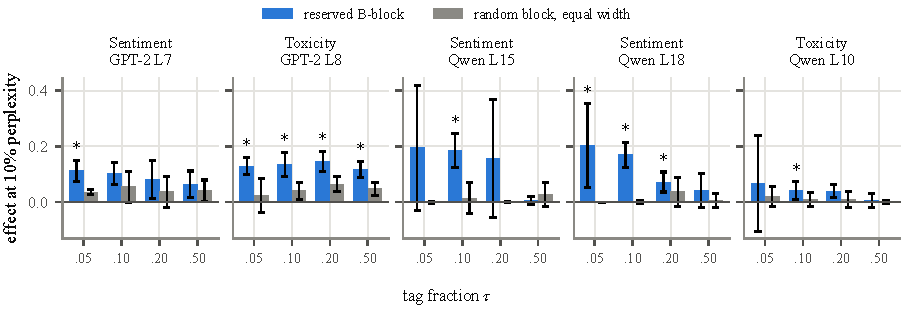
\includegraphics[width=0.95\linewidth]{figures/fig_block.pdf}
  \caption{Reserved bucket against a random block of the same size: effect at a \budget\%
  perplexity budget (mean $\pm$ 95\% CI over seeds; $^{*}\,p<0.05$).}
  \label{fig:block}
\end{figure}

\begin{figure}[H]
  \centering
  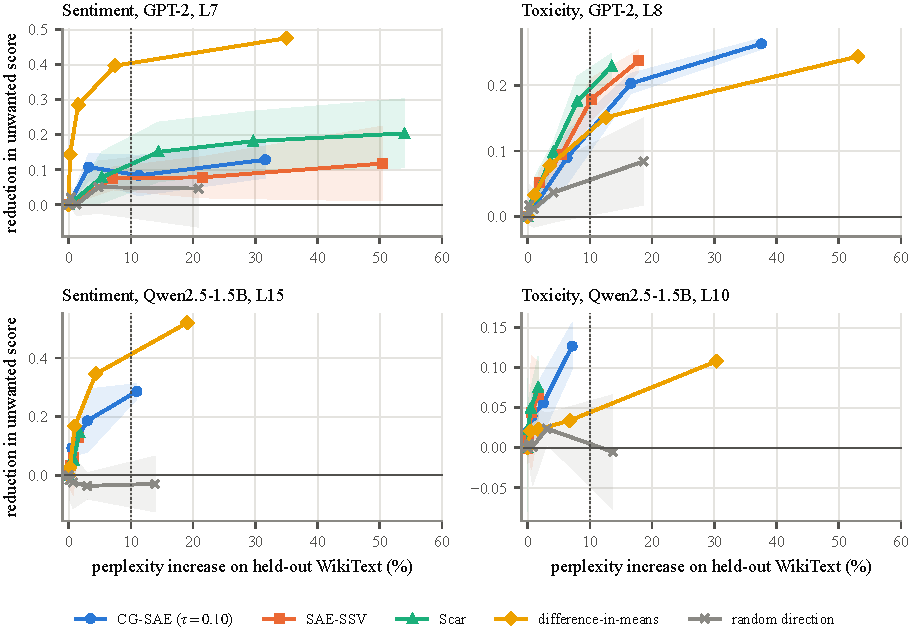
\includegraphics[width=0.95\linewidth]{figures/fig_tradeoff.pdf}
  \caption{Effect against fluency cost for every method. The dotted line is the \budget\% budget at
  which methods are compared.}
  \label{fig:tradeoff}
\end{figure}

\subsection{Which layer?}
\label{sec:layers}
A common shortcut is to edit the layer where a linear probe~\cite{belinkov2022probing,hewitt2019control}
best detects the concept. We scanned every layer for both models and concepts. In
\layerDisagree{} of \layerScans{} scans, the best layer for \emph{detecting} the concept was not the
best layer for \emph{steering} it. On GPT-2 sentiment, the probe picks layer \layerGptProbe{} but
steering works best at layer \layerGptSteer{}; using the probe's choice loses \layerGptLoss\% of the
efficiency (Figure~\ref{fig:layers}). We therefore chose layers by steering efficiency.

\begin{figure}[H]
  \centering
  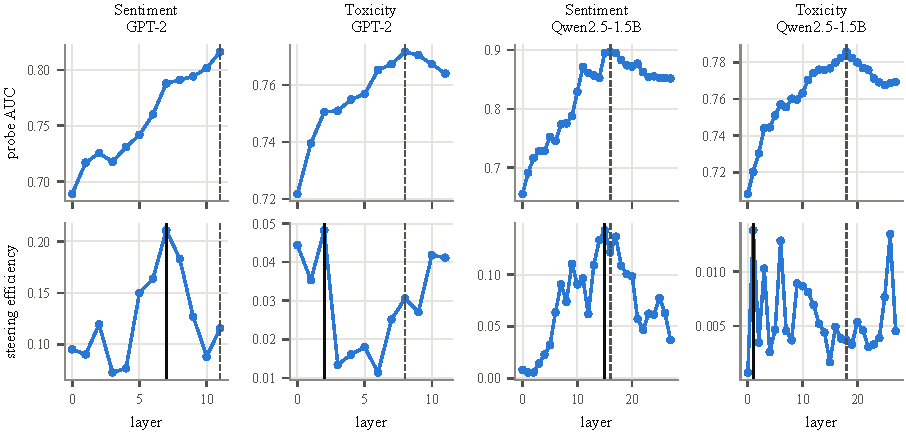
\includegraphics[width=0.95\linewidth]{figures/fig_layers.pdf}
  \caption{Layer scans. Top: linear-probe AUC per layer. Bottom: steering efficiency (effect per
  unit of perplexity cost). Dashed: best probe layer; solid: best steering layer.}
  \label{fig:layers}
\end{figure}

%=====================================================================
\section{Comparison with state-of-the-art methods}
\label{sec:sota}

Published numbers from other papers are not directly comparable to ours, because they use different
models, datasets, judges and edit strengths. We therefore re-implemented the strongest
representatives of each family in \emph{our} pipeline and compared all of them under identical
conditions: same frozen model and layer, same prompts and judge, same SAE width and sparsity, and the
same \budget\% fluency budget.

\subsection{Conceptual comparison}
\begin{center}
\small
\begin{tabularx}{\linewidth}{>{\raggedright\arraybackslash}p{3.9cm}cccc>{\raggedright\arraybackslash}X}
\toprule
Method & \shortstack{Location fixed\\before training} & \shortstack{Removes\\weights} & \shortstack{Explicit place\\for shared features} & \shortstack{Needs\\labels} & Note\\
\midrule
ActAdd~\cite{turner2023actadd}, CAA~\cite{rimsky2024caa} & no & no & no & pairs & run-time direction\\
ITI~\cite{li2023iti}, RepE~\cite{zou2023repe} & no & no & no & yes & run-time direction\\
Refusal direction~\cite{arditi2024refusal} & no & optional & no & yes & one direction\\
SAE + post-hoc selection (SAE-SSV~\cite{he2025saessv}) & no & no & no & yes & search after training\\
SCAR~\cite{harle2024scar} & yes (1 unit) & no & no & yes & one conditioned unit\\
Gradient routing~\cite{cloud2024gradient} & yes & yes & implicit & yes & masks gradients\\
\textbf{Ours (buckets + buffer)} & \textbf{yes} & \textbf{yes} & \textbf{yes} & yes & activation penalty; works in-model and in SAEs\\
\bottomrule
\end{tabularx}
\end{center}

Our method is the only one in this list that fixes the location in advance, deletes real weights,
and reserves an explicit, unpenalised region for features shared by both behaviours. In gradient
routing, parameters that are not masked receive gradients from all data and therefore play this role
implicitly; it has no tunable buffer and no experiment isolating its effect.

\subsection{Quantitative comparison under matched conditions}

\begin{table}[H]
\centering
\caption{Reduction in the judged unwanted score at a \budget\% fluency budget (higher is better;
mean over seeds). $p$: paired test against difference-in-means. All SAE arms were fixed in advance,
with no best-arm selection.}
\label{tab:sota}
\small
\begin{tabular}{lcccc}
\toprule
& \multicolumn{2}{c}{GPT-2} & \multicolumn{2}{c}{Qwen2.5-1.5B}\\
\cmidrule(lr){2-3}\cmidrule(lr){4-5}
Method & sentiment & toxicity & sentiment & toxicity\\
\midrule
Difference-in-means (ActAdd/CAA-style) & \textbf{\dimGptSent} & \dimGptTox & \textbf{\dimQwenSent} & \dimQwenTox\\
SCAR-style single unit & \scarGptSent{} ($p\,\scarPGptSent$) & \textbf{\scarGptTox}{} ($p=\scarPGptTox$) & \scarQwenSent{} ($p\,\scarPQwenSent$) & \scarQwenTox{} ($p=\scarPQwenTox$)\\
Ours: bucketed SAE & \cgGptSent{} ($p\,\cgPGptSent$) & \cgGptTox{} ($p=\cgPGptTox$) & \cgQwenSent{} ($p=\cgPQwenSent$) & \textbf{\cgQwenTox}{} ($p=\cgPQwenTox$)\\
\bottomrule
\end{tabular}
\end{table}

\textbf{Reading the comparison.}
\begin{itemize}
  \item \textbf{Toxicity.} No SAE method is significantly worse than difference-in-means, and on
  Qwen2.5-1.5B our bucketed SAE is significantly better: \cgQwenTox{} against \dimQwenTox, roughly
  $2.9\times$ the effect at the same fluency cost ($p=\cgPQwenTox$). On GPT-2 the SCAR-style unit is
  best. Across both models, \dimToxSAEbetter{} of \dimToxTotal{} toxicity comparisons significantly
  favour an SAE method and none favour difference-in-means.
  \item \textbf{Sentiment.} Difference-in-means is clearly best, ahead of every SAE method in
  \dimSentSAEworse{} of \dimSentTotal{} comparisons. Sentiment is close to a single linear direction
  in these models, which is exactly the case where one direction is hard to beat.
  \item \textbf{Against a normal SAE with post-hoc selection (SAE-SSV-style).} At the same
  intervention width, training the SAE with buckets helps on Qwen2.5-1.5B (\vsSSVqwenPositive{} of
  \vsSSVqwenTotal{} differences positive, \vsSSVqwenSig{} significant) but not on GPT-2
  (\vsSSVgptSig{} of \vsSSVgptTotal), so the benefit appears with model size.
  \item This concept-dependent ranking agrees with an independent comparison of SAE and
  difference-based steering~\cite{xie2025comparative}.
\end{itemize}

\textbf{What only our method provides.} None of the steering baselines removes anything from the
model: they act at run time and the knowledge stays in the weights. The in-model result of
Section~\ref{sec:exp2} (selective perplexity loss after deleting real weights, in all seeds, with a
random-deletion control) has no counterpart among these methods; the closest is gradient
routing~\cite{cloud2024gradient}, from which we differ by the explicit buffer and its measured
effect (Section~\ref{sec:exp1}).

%=====================================================================
\section{Design decisions and rationale}
\label{sec:decisions}

\begin{center}
\small
\begin{tabularx}{\linewidth}{>{\raggedright\arraybackslash}p{3.6cm}>{\raggedright\arraybackslash}X}
\toprule
Decision & Reason\\
\midrule
Reserve buckets \emph{before} training & Removal becomes deletion by address; no search afterwards~\cite{harle2024scar,he2025saessv}.\\
Add a neutral buffer & Shared features need a place; without it specificity falls to chance (Exp.~1).\\
Contrastive penalty on shares & Squared-mean penalty is inert under sparsity and is satisfied by silence (Sec.~\ref{sec:penform}).\\
$0<\uptau\le\frac12$, mostly $\uptau=0.1$ & Two buckets must fit; $0.1$ leaves a large buffer ($\uprho=4$), which worked best.\\
$\uplambda=3$ inside GPT-2 & $\uplambda=1$ formed no buckets; $\uplambda=10$ cost \ghWikiCostPct\% fluency.\\
Labels only in the loss & The model must work normally on unlabelled text at test time.\\
Always compare with a random bucket & Deleting any units hurts; only the ratio shows targeting.\\
Perplexity for knowledge, classifier for behaviour & They measure different things and turned out to disagree.\\
TopK SAE~\cite{gao2024scaling} & Exact, equal sparsity for every compared SAE.\\
Difference-of-decodes edit & $\upalpha=0$ is exactly no change; cost is of the edit alone.\\
Matched \budget\% fluency budget & Breaking the model is not removing a behaviour.\\
Difference-in-means baseline~\cite{rimsky2024caa,turner2023actadd} & Simple, strong; any new method must beat it.\\
Report routing, not leakage & Leakage rewards dead buckets ($r=\leakRoutingCorr$).\\
Choose layers by steering scan & Probe-best layer differed in \layerDisagree{}/\layerScans{} scans.\\
Greedy decoding & Removes sampling noise from behaviour measurements.\\
Sign test, Holm correction~\cite{holm1979} & Many settings are tested; avoid false positives.\\
GPT-2 and Qwen2.5-1.5B & Two model families and two scales within our compute budget.\\
IMDB and RealToxicityPrompts~\cite{maas2011imdb,gehman2020rtp} & Standard public datasets with labels.\\
\bottomrule
\end{tabularx}
\end{center}

%=====================================================================
\section{Limitations and error analysis}
\label{sec:limits}
\begin{enumerate}
  \item \textbf{Knowledge moves, behaviour does not reliably follow.} Perplexity shows selective
  removal, but the model's generations became less negative clearly only in the small
  from-scratch model (2 seeds).
  \item \textbf{Relearning.} 100 steps of retraining bring the behaviour back as easily as after a
  random deletion. This is a known weakness of unlearning by deletion.
  \item \textbf{Fluency cost.} Training with the penalty costs \gtWikiCostPct\% WikiText perplexity at
  $\uplambda=3$ and \ghWikiCostPct\% at $\uplambda=10$.
  \item \textbf{Mixed SAE results.} The bucketed SAE beats a normal SAE on Qwen but not on GPT-2, and
  difference-in-means is better on sentiment.
  \item \textbf{Scale.} Small models (GPT-2 small, a 1.5B model for SAEs), 2--3 seeds for language
  models, two concepts. Larger models and more seeds are needed.
  \item \textbf{Proxy for harm.} In-model experiments use negative sentiment as a stand-in for harmful
  behaviour; toxicity appears only in the SAE experiments.
\end{enumerate}

\textbf{Next steps.} Combine bucket deletion with a behaviour-level objective; test several
buckets for several behaviours at once; test larger models; compare directly with gradient
routing~\cite{cloud2024gradient}; test safety behaviours such as refusal~\cite{arditi2024refusal}.

%=====================================================================
\section{FAQ}
\label{sec:qa}

\textbf{Q: How is this different from gradient routing?} Gradient routing~\cite{cloud2024gradient}
localises a capability by masking which parameters receive gradients from which data. We leave
gradients untouched and add an activation-level penalty, with an explicit neutral buffer for
shared features, and we apply the same idea both inside a model and inside an SAE.

\textbf{Q: How is it different from SCAR?} SCAR~\cite{harle2024scar} ties a concept to a single
SAE feature. We reserve a whole bucket and a buffer, and we show the buffer is what makes deletion
targeted.

\textbf{Q: Why not just use difference-in-means steering?} On sentiment it is indeed better, and we
report that. On toxicity SAEs work better. Our main contribution is the in-model deletion, which
steering does not provide: steering is applied at run time and the knowledge stays in the weights.

\textbf{Q: Is the knowledge really gone?} By perplexity, it is selectively reduced. But it can be
relearned quickly, so we do not claim permanent removal.

\textbf{Q: Why is 0.91 called chance?} Specificity is a ratio against a random deletion of the same
size. $1$ means ``exactly as damaging as random''; $0.91$ is slightly below, i.e.\ no targeting.

\textbf{Q: Why did leakage fail?} Because a silent bucket has zero leakage. See
Section~\ref{sec:leakage}.

\textbf{Q: Why should the same idea work in an SAE and inside a model?} Both are layers of units
with non-negative activity, and the penalty only needs the shares $s_{\Wb},s_{\Ub}$. Only the
deletion step differs.

%=====================================================================
\section{Glossary}
\begin{description}[leftmargin=0pt,itemsep=1pt]
  \item[Bucket] A fixed set of units reserved for one behaviour ($\Wb$ or $\Ub$).
  \item[Neutral buffer ($\Nb$)] Units that are never penalised or deleted; home for shared features.
  \item[$\uptau$] Fraction of units in each bucket; $0<\uptau\le\frac12$.
  \item[$\uplambda$] Weight of the penalty in the training loss.
  \item[Share $s_S$] Fraction of a token's total activity that falls in set $S$.
  \item[Routing $R$] How much more of the activity $\Ub$ carries on unwanted than on wanted text.
  \item[Specificity $S$] Damage from deleting $\Ub$ divided by damage from deleting a random set.
  \item[Perplexity] How surprised the model is by a text; lower is better.
  \item[SAE] Sparse autoencoder: rewrites a hidden vector as a few active features.
  \item[FVU] Fraction of variance unexplained; reconstruction error of an SAE.
  \item[TopK] Keep the $k$ largest activations, zero the rest.
  \item[Steering] Adding or removing a direction in the hidden state at run time.
  \item[Superposition] Many concepts sharing the same neurons.
\end{description}

\bibliographystyle{IEEEtran}
\bibliography{IEEEabrv,references}

\end{document}
